\documentclass[a4paper]{report}

\usepackage[english]{babel}
\usepackage{caption}
\usepackage{subcaption}
\usepackage{listings, color}
\usepackage{graphicx}
\usepackage{chngpage}
\usepackage{longtable}
\usepackage{float}
\usepackage{comment}
\usepackage[usenames,dvipsnames]{xcolor}
\usepackage{epstopdf}
\usepackage{titlesec}
\usepackage{pdfpages}
\usepackage{wrapfig}
\usepackage{url}
\usepackage{hyperref}
\usepackage[nodisplayskipstretch]{setspace}
\usepackage[top=2cm,bottom=2.5cm]{geometry}
\usepackage{amsmath}
\usepackage{caption} 
\usepackage{natbib}
\usepackage[nottoc,numbib]{tocbibind}
\usepackage{xpatch}

\definecolor{dkgreen}{rgb}{0,0.6,0}
\definecolor{gray}{rgb}{0.5,0.5,0.5}
\definecolor{mauve}{rgb}{0.58,0,0.82}

\lstset{frame=tb,
  language=Matlab,
  aboveskip=3mm,
  belowskip=3mm,
  showstringspaces=false,
  columns=flexible,
  basicstyle={\small\ttfamily},
  numbers=left,
  numberstyle=\tiny\color{gray},
  keywordstyle=\color{black},
  commentstyle=\color{dkgreen},
  stringstyle=\color{mauve},
  breaklines=true,
  breakatwhitespace=true
  tabsize=3
}

\newcommand{\tab}{\hspace*{2em}}
\titleformat{\chapter}{\normalfont\huge\bf}{\thechapter.}{20pt}{\huge\bf}

\newcommand\fnurl[2]{%
  \href{#2}{#1}\footnote{\url{#2}}%
}


\xpatchcmd{\itemize}
  {\def\makelabel}
  {\setlength{\itemsep}{0em}\def\makelabel}
  {}
  {}

\begin{document} 

\begin{titlepage}

\newcommand{\HRule}{\rule{\linewidth}{0.5mm}} % Defines a new command for the horizontal lines, change thickness here

\center % Center everything on the page
 
%----------------------------------------------------------------------------------------
%	HEADING SECTIONS
%----------------------------------------------------------------------------------------

\textsc{\LARGE Group 7}\\[1.5cm] % Name of your university/college

%----------------------------------------------------------------------------------------
%	TITLE SECTION
%----------------------------------------------------------------------------------------

\HRule \\[0.4cm]
{ \huge \bfseries Assignment 3}\\[0.4cm] % Title of your document
\HRule \\[4cm]
 
%----------------------------------------------------------------------------------------
%	AUTHOR SECTION
%----------------------------------------------------------------------------------------

\begin{minipage}{0.5\textwidth}
\emph{Authors:}\\     
Emilie de Bree - 4247558\\
Toine Hartman - 4305655\\
Jeffrey Helgers - 4318749 \\
Jim Hommes - 4306090\\
Joost Pluim - 4162269 \\
Matthijs Verzijl - 4282604\\\\
\emph{Supervisor:} \\
Alberto Bacchelli \\\\
\emph{Teaching Assistant:} \\
Aaron Ang\\
\end{minipage}\\[4cm]


%----------------------------------------------------------------------------------------
%	LOGO SECTION
%----------------------------------------------------------------------------------------


\includegraphics[width=100mm]{logo.jpg}\\[1cm] % Include a department/university logo - this will require the graphicx package

%----------------------------------------------------------------------------------------
%	DATE SECTION
%----------------------------------------------------------------------------------------

{\large \today}\\[3cm] % Date, change the \today to a set date if you want to be precise

\vfill % Fill the rest of the page with whitespace

\end{titlepage}
\tableofcontents
\thispagestyle{empty}
\setcounter{page}{0}
\chapter{The Core}
\section{Question 1}

``Following the Responsibility Driven Design, start from your requirements (without considering your implementation) and derive classes, responsibilities, and collaborations (use CRC cards). Describe each step you make. Compare the result with your actual implementation and discuss any difference (e.g., additional and missing classes).'' \\

\noindent As a recap we will start by providing our requirements: 
\begin{itemize}
    \item The game shall have a single level to play.
    \item The game shall show a game over screen when the player dies.
  \item The game shall have a field where the character and monsters can move around.
    \item The player shall have the ability to win the game when they have killed all the monsters.
  \item The player shall lose the game when a monster touches the character.
    \item The player's character must be able to move around horizontally.
    \item The player's character must be able to jump, both straight up and diagonally.
    \item The player's character shall be able to shoot bubbles.
    \item The monsters shall walk around horizontally, and when they hit a wall they will change direction. 
  \item A monster shall be trapped in a bubble when the player shoots a bubble at it.
  \item A monsters shall die when it is caught in a bubble and the character collides with that bubble.
   \item The game shall have a start up screen.
   \item The game shall have multiple levels to play on.
   \item The game shall keep a track of the player's score.
   \item The game shall have the ability to pause.
   \item The game shall have the ability to unpause after the pause button have been pressed.
   \item The game shall have the ability to stop, which closes the game.
   \item The game shall have a help screen that will inform the player about the controls and powerups.
   \item The player shall have the ability to start a new game.
   \item The player shall have multiple lives.
   \item The player shall lose a life, when a monster touches the character. 
   \item The monsters shall be able to drop items when they die.
   \item The player shall have the ability to pick up items which will increase their score.
   \item The powerups shall increase the speed of the bubble, the distance the bubble travels or the walking speed of the character.\\\\\\
\end{itemize}

\noindent Next step is to derive all necessary classes from the requirements. Useful to do this is by selecting every noun in the requirements. 
\begin{itemize}
    \item LevelController
    \item Level
    \item Wall
    \item Character
    \item Sprite
    \item Monster
    \item Input
    \item Bubble
    \item PowerUp
\end{itemize}

\noindent Since we now have all classes present, we can start constructing our CRC cards

\begin{table}[h!]
\centering
\label{crc_levelcontroller}
\begin{tabular}{|l|l|}
\hline
\multicolumn{2}{|l|}{\textbf{LevelController}} \\ \hline
\multicolumn{2}{|l|}{Superclass(es):} \\ \hline
\multicolumn{2}{|l|}{Subclass(es): Level, Player} \\ \hline
createLvl               & Level \\ \hline
createPlayer            & Player \\ \hline
startLvl                & Level \\ \hline
winLvl                  & Level \\ \hline
\end{tabular}
\caption{CRC card: LevelController}
\end{table}

\begin{table}[h!]
\centering
\label{crc_level}
\begin{tabular}{|l|l|}
\hline
\multicolumn{2}{|l|}{\textbf{Level}} \\ \hline
\multicolumn{2}{|l|}{Superclass(es):} \\ \hline
\multicolumn{2}{|l|}{Subclass(es): Wall} \\ \hline
initiateLevel           & Level \\ \hline
initiateWalls           & Wall \\ \hline
initiateSprite          & Sprite \\ \hline
initiateMonsters        & Monster \\ \hline
\end{tabular}
\caption{CRC card: Level}
\end{table}

\begin{table}[h!]
\centering
\label{crc_wall}
\begin{tabular}{|l|l|}
\hline
\multicolumn{2}{|l|}{\textbf{Wall}} \\ \hline
\multicolumn{2}{|l|}{Superclass(es):} \\ \hline
\multicolumn{2}{|l|}{Subclass(es):} \\ \hline
setX           & Integer \\ \hline
setY           & Integer\\ \hline
\end{tabular}
\caption{CRC card: Wall}
\end{table}

\begin{table}[h!]
\centering
\label{crc_sprite}
\begin{tabular}{|l|l|}
\hline
\multicolumn{2}{|l|}{\textbf{Sprite}} \\ \hline
\multicolumn{2}{|l|}{Superclass(es):} \\ \hline
\multicolumn{2}{|l|}{Subclass(es): Character, Monster} \\ \hline
get/setX           & Integer \\ \hline
get/setY           & Integer \\ \hline
get/setR           & Integer \\ \hline
get/setDx          & Integer \\ \hline
get/setDy          & Integer \\ \hline
get/setDr          & Integer \\ \hline
get/setCanMove     & Boolean \\ \hline
get/setImagePath   & String \\ \hline
get/setWidth       & Integer \\ \hline
get/setHeight      & Integer \\ \hline
\end{tabular}
\caption{CRC card: Sprite}
\end{table}

\begin{table}[h!]
\centering
\label{crc_character}
\begin{tabular}{|l|l|}
\hline
\multicolumn{2}{|l|}{\textbf{Character}} \\ \hline
\multicolumn{2}{|l|}{Superclass(es): Sprite} \\ \hline
\multicolumn{2}{|l|}{Subclass(es): Bubble, Input} \\ \hline
moveLeft            & Input \\ \hline
moveRight           & Input \\ \hline
fireWeapon          & Input \\ \hline
die                 & - \\ \hline
isDead              & Boolean \\ \hline
\end{tabular}
\caption{CRC card: Character}
\end{table}

\begin{table}[h!]
\centering
\label{crc_monster}
\begin{tabular}{|l|l|}
\hline
\multicolumn{2}{|l|}{\textbf{Monster}} \\ \hline
\multicolumn{2}{|l|}{Superclass(es): Sprite} \\ \hline
\multicolumn{2}{|l|}{Subclass(es):} \\ \hline
get/setSpeed            & Integer \\ \hline
checkCollision          & -\\ \hline
get/setDirection        & String\\ \hline
isCaught                & Boolean \\ \hline
isDead                  & Boolean \\ \hline
\end{tabular}
\caption{CRC card: Monster}
\end{table}

\begin{table}[h!]
\centering
\label{crc_input}
\begin{tabular}{|l|l|}
\hline
\multicolumn{2}{|l|}{\textbf{Input}} \\ \hline
\multicolumn{2}{|l|}{Superclass(es):} \\ \hline
\multicolumn{2}{|l|}{Subclass(es):} \\ \hline
moveUp          & -\\ \hline
moveDown        & - \\ \hline
moveLeft        & -\\ \hline
moveRight       & -\\ \hline
fireWeapon      & - \\ \hline
\end{tabular}
\caption{CRC card: Input}
\end{table}

\begin{table}[h!]
\centering
\label{crc_bubble}
\begin{tabular}{|l|l|}
\hline
\multicolumn{2}{|l|}{\textbf{Bubble}} \\ \hline
\multicolumn{2}{|l|}{Superclass(es):} \\ \hline
\multicolumn{2}{|l|}{Subclass(es):} \\ \hline
ableToCatch           & - \\ \hline
move           & -\\ \hline
\end{tabular}
\caption{CRC card: Bubble}
\end{table}

\begin{table}[h!]
\centering
\label{crc_powerup}
\begin{tabular}{|l|l|}
\hline
\multicolumn{2}{|l|}{\textbf{PowerUp}} \\ \hline
\multicolumn{2}{|l|}{Superclass(es):} \\ \hline
\multicolumn{2}{|l|}{Subclass(es):} \\ \hline
get/setAbleToPickup           & Boolean \\ \hline
\end{tabular}
\caption{CRC card: PowerUp}
\end{table}

\newpage
When comparing this with our actual implementation we notice a couple things:
\begin{itemize}
\item In our actual implementation, the classes Monster and Sprite have their own superclasses.
\item The class PowerUp hasn\'t been implemented yet. 
\item Some of the classes are named differently, which can make easy explaining of classes harder. 
\item The class Sprite (our called Player in the implementation), has more methods, cause there are multiple variables defined which we didn't think of in the CRC cards. Examples are a counter variable to count the bubbles, an array of all the bubbles a player fired, a variable to check whether the player can jump. 
\end{itemize}
\subsection{Exercise 1.2}
``Following the Responsibility Driven Design, describe the main classes you implemented in your project in terms of responsibilities and collaborations''

\subsection{Launcher}
Responsibility: \\
The Launcher launches the game by loading the StartorEndController. \\
Collaborations: \\
The Launcher collaborates with the StartorEndController. 

\subsubsection{StartorEndController}
Responsibility: \\
The StartorEndController starts the game, or ends it. \\
Collaborations: \\
The StartorEndController collaborates with LevelController toe load the Level which will be placed. 

\subsubsection{LevelController}
Responsibilities: \\
The LevelController-class is responsible for handling interaction between a Level and Players. It is also runs the gameLoop which renders the game every frame. Therefor it is also able to pause the game, win a game and go to a next Level. \\
Collaborations: \\
The LevelController-class collaborates with a Level and the Players.

\subsubsection{ScreenController}
Responsibilities: \\
The ScreenController is responsible for drawing everything on a screen. \\
Collaborations: \\
The ScreenController works together with the LevelController as well as SpriteBase to draw every sprite on the screen. 

\subsubsection{Level}
Responsibilities: \\
The Level-class is responsible for constructing the level a customer plays. A level has to be created from loading a text-file in which is defined where to place the walls and the monsters. \\
Collaborations: \\
The Level-class collaborates with SpriteBase to display every element in the Level.  

\subsubsection{SpriteBase}
Responsibilities: \\
Every element in Level has certain standard attributes such as an x,y coordinate, but also the speed in every direction and an image. All of these attributes are defined in SpriteBase. \\
Collaborations: \\
Depending on the kind of SpriteBase, the customer must be able to perform input. Therefor the SpriteBase collaborates with Input. 

\subsubsection{Input}
Responsibilities: \\
The Input class catches all input performed by the customer. The class makes sure that when a customer presses one of the keys allowed the desired action is performed and when the key is released the action stops. \\
Collaborations: \\
The only object which can be moved by the customer is the Player class. Therefor this is the only class with which the Input class collaborates. 

\subsubsection{Non-main classes}
The classes GravityObject, Bubble, Wall, Monster, Player and Walker are all (direct or indirect) extensions of SpriteBase. Therefor they can be removed. Settings is a class with only static information and can therefor also be merged in a controller. 
\chapter{The Core: Question 3}
``Why do you consider the other classes as less important? Following the Responsibility Driven Design,
reflect if some of those non-main classes have similar/little responsibility and could be changed,
merged, or removed. If so, perform the code changes; if not, explain why you need them''\\
\\
The classes that are considered less important are:
\begin{itemize}
	\item GameOverController
	\item WinController
	\item Settings
	\item Player
	\item Monster
	\item Walker
	\item GravityObject
	\item Bubble
	\item Wall
\end{itemize}
\\
The GameOverController and WinController are important because they control the screen when you win or lose, But these classes are almost the same. They both create a screen with a Play Again and a Quit button. The only differences between these classes are the picture on the screen and the way they are called. The WinController is called when all the monsters are killed, and the GameOverController when the character touches a monster. We have removed these two classes, and created one class new class: StartOrEndController. This controller creates a screen with the two buttons, with a different image when you win or lose.\\
\\
The class Settings is a class that contains information about the game, like speed of monsters, bubbles and the player. This class makes the programming more clear.
\\
The other classes are all extensions from SpriteBase. All these classes are necessary to run the program correctly. The classes GravityObject, Bubble and Wall are direct extensions from SpriteBase.\\
The GravityObjects are all the object that can move in different directions in the level.\\
The Walls are the objects that can't collide with other sprites.\\
The bubbles are the bubbles that move in a specific direction, a few steps to the left or right and then they move up. These bubbles are shoot by a player and can catch the monsters.\\
The classes Monster and Player are extensions from GravityObject. The difference between these classes is that the monsters move around freely, and the player moves around by key presses. At the moment is it possible to remove the class Monster, because there is only one extension from this class: Walker. Which represent the monsters that walk around the field. But we won't remove the class Monster because in the future we may want to create different types of monster, for instance monsters that fly or can shoot.
\chapter{The Core: Question 4}

``Draw the class diagram of the aforementioned main elements of your game (do not forget to use elements such as parametrised classes or association constrains, if necessary).''

\begin{figure}[h]
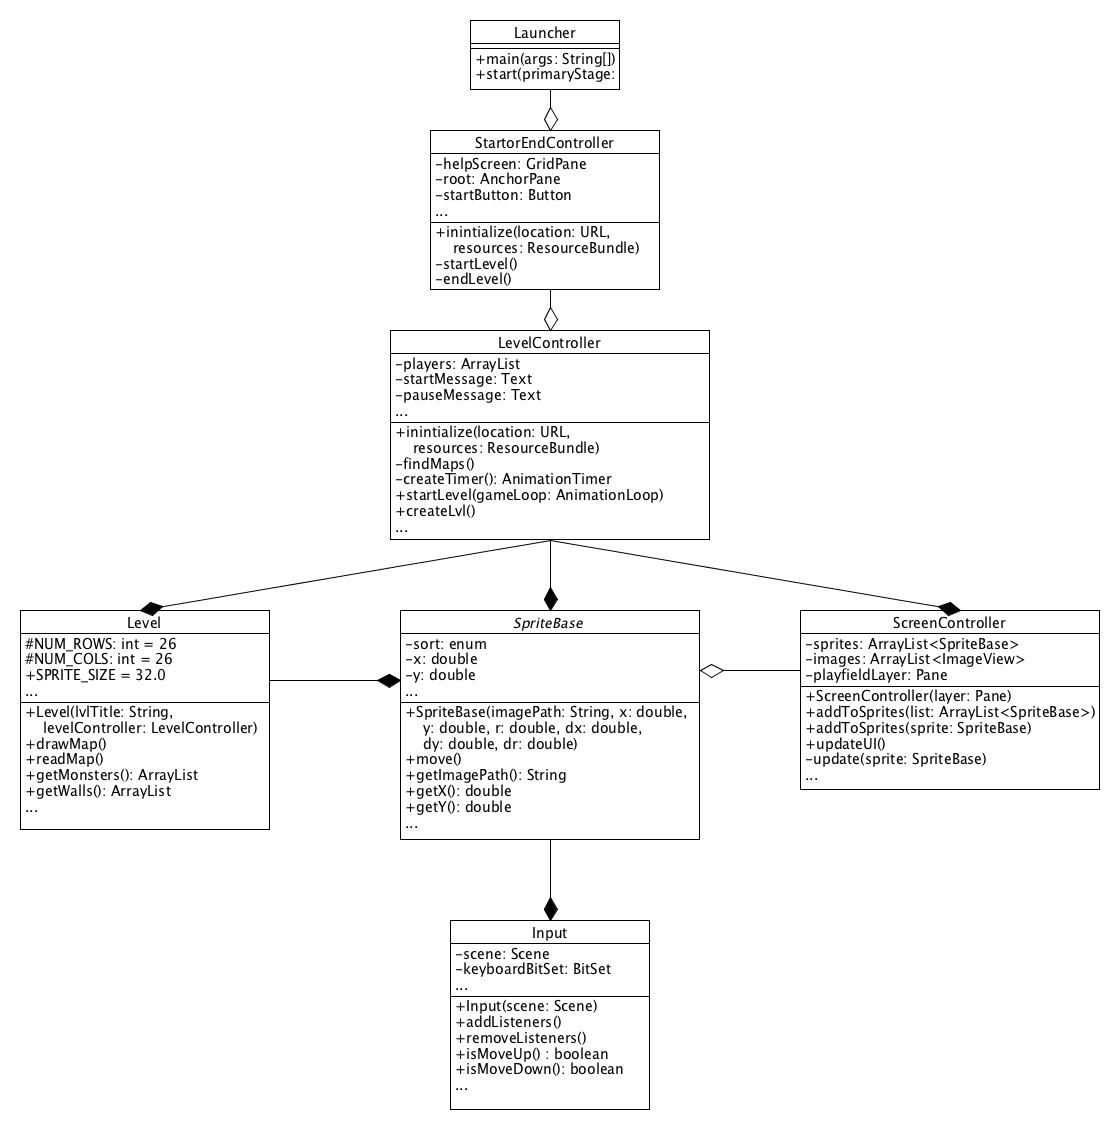
\includegraphics[width=\textwidth]{classDiagramsMain}
\end{figure}
\section{Question 5}
``Draw the sequence diagram to describe how the main elements of your game interact (consider asynchrony and constraints, if necessary)''

\begin{figure}[h]
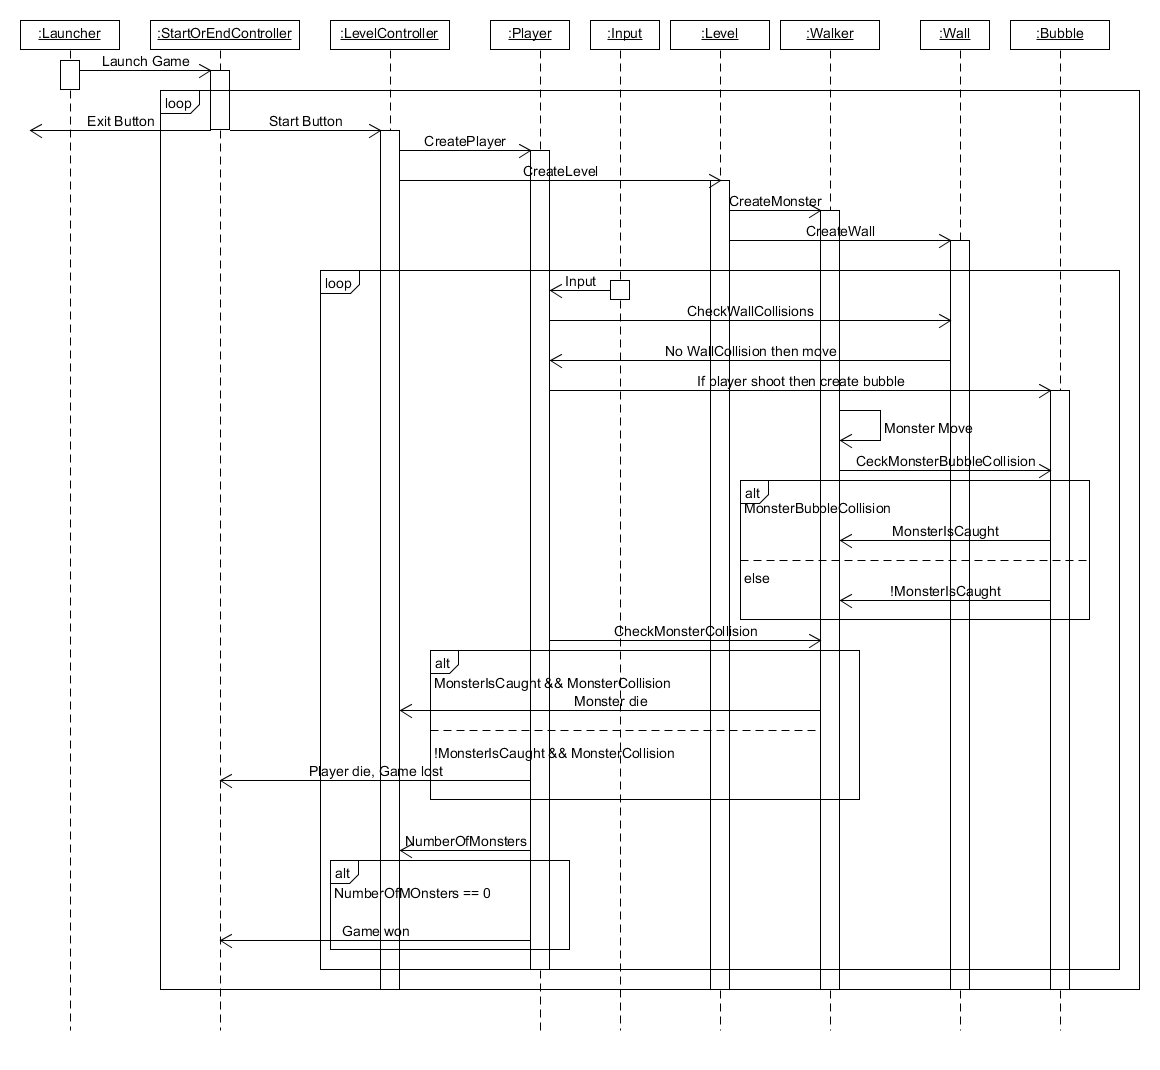
\includegraphics[width=\textwidth]{SequenceDiagram}
\end{figure}

\chapter{UML in practice}
\section{Question 1}
``What is the difference between aggregation and composition? Where are composition and aggregation
used in your project? Describe the classes and explain how these associations work.''

The difference between aggregation and composition is that in composition class A owns class B (or contains). While in aggregation, class A uses class B (or consists of), so the classes are independent of each other. 
\\\\
In our project there are both examples of aggregation as well as composition, as listed below:

\begin{itemize}
\itemsep0em 
\item Aggregation can be found between:
	\begin{itemize}
	\itemsep0em
	\item \textbf{Launcher} and \textbf{StartController}; Launcher uses the StartController to be able to start the game.	
	\item \textbf{StartOrEndController} and \textbf{StartController}; StartOrEndController uses the StartController to be able to start the game again.
	\item \textbf{StartController} and \textbf{LevelController}; StartController uses the LevelController to be able to create the level. 
	\item \textbf{LevelController} and \textbf{StartOrEndCOntroller}; LevelController uses the StartOrEndController to be able to restart the game after the player has won or lost.
	\item \textbf{ScreenController} and \textbf{SpriteBase}; ScreenController uses the SpriteBase to be able to create the sprites on the screen, when playing the game.
	\item \textbf{Level} and \textbf{Settings}; Level uses the Settings to get measurements for the level.
	\item \textbf{Bubble} and \textbf{Settings}; Bubble uses the Settings to get the measurements for the bubbles that will be shot. 
	\item \textbf{Player} and \textbf{Settings}; Player uses the Settings to get the measurements for the character that the player will be playing.
	\end{itemize}
\item Composition can be found between:
	\begin{itemize}
	\itemsep0em
	\item \textbf{LevelController} and \textbf{ScreenController}; LevelController can not exist without the use of the ScreenController as the ScreenController controls what happens on the screen during a level.
	\item \textbf{LevelController} and \textbf{SpriteBase}; LevelController owns SpriteBase because without SpriteBase the levels can not be created to be controller by the controller.
	\item \textbf{LevelController} and \textbf{Level}; LevelController owns Level because without the Level class the LevelController can not create the levels for the game to be played on. 
	\item \textbf{Level} and \textbf{SpriteBase}; Level contains SpriteBase because without SpriteBase the levels can not be created as the SpriteBase is used to create all the sprites in a level.
	\item \textbf{Player} and \textbf{Input}; Player owns Input because without Input the player can not exist to be played.
	\end{itemize}
\end{itemize} 

\section{Question 2}

``Is there any parametrized class in your source code? If so, describe which classes, why they are
parametrized, and the benefits of the parametrization. If not, describe when and why you should use
parametrized classes in your UML diagrams.''
\\
\\
In our project we haven't implemented any parameterised classes, but we do use a parameterised class from java.util, the ArrayList. \\
\\
A parameterised class should be in the UML diagram when you have implemented a parameterised class in your source code. The paramaterised class from java.util that we used is also visible in the UML diagram, but not as a parameterised class, as a attribute from a different class.\\
\\
You should use a parameterised class when you don't know with wich generic type the class will be used. With the parameter you can define the type on wich the class will operate.\\
\\
The UML diagram shows a parameterised class with a dotted box over the right corner of a normal class. In this box goes the parameter for that specific class. 
\chapter{UML in practice: Question 3}

\begin{figure}[h]
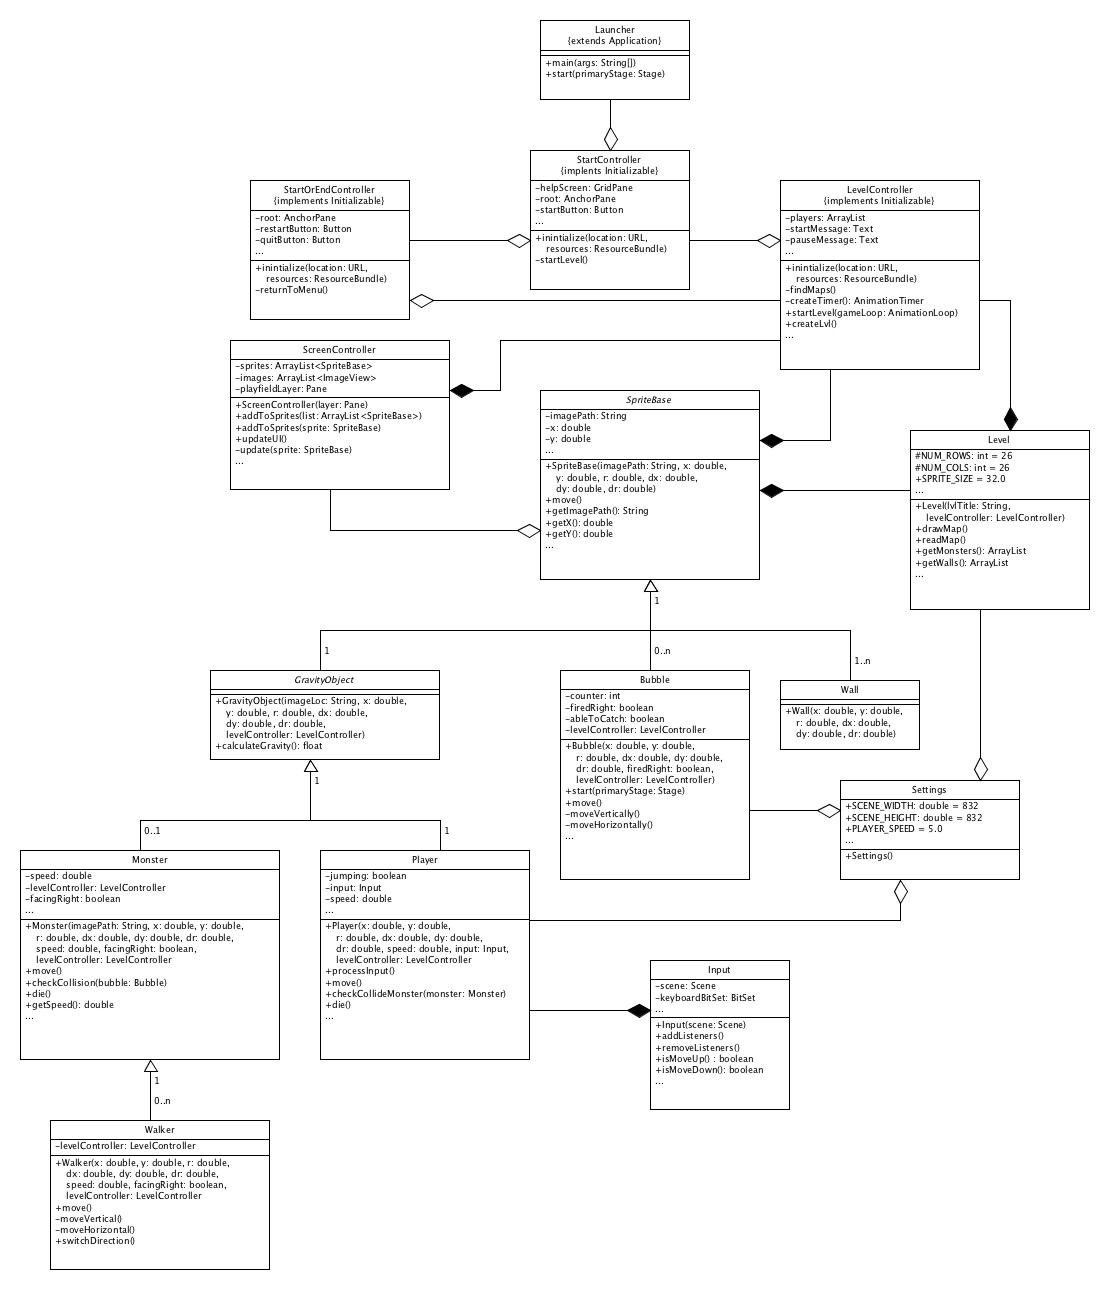
\includegraphics[width=\textwidth]{classDiagramsUML_3.jpg}
\caption{The class diagram for the whole project.}
\end{figure}

\noindent The hierarchies that can be seen have been chosen to stop the code from becoming too complex, and to allow both the programmers and developers, as well as anyone who would be looking at the code to have a better understanding of how the code is set up. The hierarchies were also created in this way, to insure that no class would get too long.
\\
\noindent The following hierarchies can be seen in the class diagram:
\begin{itemize}
\itemsep0em 
\item There is Polymorphism between SpriteBase (the super class) and its three sub classes GravityObject, Bubble and Wall.
\item There is Polymorphism between GravityObject (the super class) and its two sub classes Monster and Player.
\item There is Is-a between Monster (the super class) and its sub class Walker.\\
\end{itemize} 

\noindent The hierarchies work well because they aren't too complex and because they allow each of the components of the game to be created without having to rewrite code multiple times.     
\chapter{Simple logging}

\section{Question 1}

``Extend your implementation of the game to support logging. The game has to log all the actions
happened during the game (e.g., player moved Tetris piece from position X to position Y ). The
logging has to be implemented from scratch without using any existing logging library. Define your
requirements and get them approved by your teaching assistant.''

See the Logger Requirements document for the logger requirements.
\section{Question 2}

``During the analysis and design phases of this extension use responsibility driven design and UML
(push to the repository a single PDF file including all the documents produced).''

\subsubsection{Introduction}
Using Responsibility Driven Design and UML this project, it is only logical to use the documentation for such an addition. That is exactly what we did. To the Responsibility Driven Design document, the following should be added:

\subsubsection{The Logger}
\textit{Responsibility:}  \\
This class will make sure that other classes are able to output information through the logger. \\
\textit{Collaborations:} \\
It should be flexible so that all the classes can collaborate with the Logger class. \\

\noindent In addition to the UML, the following class should be added:

\includegraphics[width=75mm]{loggerUML.png}

\noindent All the classes which deem it necessary to log will aggregate (filled in diamond arrow) the Logger class.
%Your text files go here
\nocite{*}
\bibliographystyle{newapa}
\end{document}